\documentclass[11pt,twoside]{book}
\usepackage{Functional/preamble}
\begin{document}
\pagestyle{empty}
\newgeometry{left=0mm,top=50mm,bottom=0mm,right=0mm}
\documentclass[]{book}
\usepackage{geometry,graphicx} % Custom margins
\usepackage[spanish]{babel}
\usepackage[T1]{fontenc}
\usepackage[dvipsnames]{xcolor} % Required for custom color
\usepackage{color,colortbl}
\usepackage[utf8]{inputenc}
\usepackage{geometry} % Custom margins
\usepackage[spanish]{babel}
\usepackage{adjustbox,dashbox}
\usepackage{array}
\usepackage{tikz,pgfplots,pgfkeys}
\usepackage{forest,mathtools,siunitx}
\usepackage{amsfonts, amssymb, amsxtra, amsmath, amsbsy}
\usepackage{newclude}
\usepackage{ifthen}
\usepackage{float}
\usepackage{fancybox}
\usepackage{graphicx,tabularx}
\usepackage{multicol,multirow}
\usepackage{enumitem} % Customising the numbered lists
\usepackage{xhfill} % Making the pink block not extend beyond the margin
\usepackage{nameref} % reference the names of the sections
\usepackage{caption,capt-of}
\usepackage[normalem]{ulem} % Dashed lines in appendix
\usepackage{ragged2e} % Ragged left
\usepackage{booktabs}
\usepackage[unboxed]{cwpuzzle}
\usepackage[colorlinks = true,linkcolor = blue]{hyperref}
\usepackage{subfiles}
\usepackage{wrapfig}
\input{insbox}
\usepackage{etoolbox}
\usepackage{mwe}
\usepackage{comfortaa}
\usepackage[T1]{fontenc}
\renewcommand*\oldstylenums[1]{{\firaoldstyle #1}}
\usepackage[T1]{fontenc}
\usepackage{pythontex}
\usepackage{polynom}
\usepackage{longdivision}


\title{Actividades}
\author{Julio C. Melchor P.\thanks{{\tt julio.melchor@rafaeldiazserdan.net}}}
\date{v1.0, \today}
%\usepackage[dvipsnames]{xcolor} % Required for custom color
\usepackage{color,colortbl}
\usepackage[utf8]{inputenc}
\usepackage{geometry} % Custom margins
\usepackage[spanish]{babel}
\usepackage{adjustbox,dashbox}
\usepackage{array}
\usepackage{tikz,pgfplots,pgfkeys}
\usepackage{forest,mathtools,siunitx}
\usepackage{amsfonts, amssymb, amsxtra, amsmath, amsbsy}
\usepackage{newclude}
\usepackage{ifthen}
\usepackage{float}
\usepackage{fancybox}
\usepackage{graphicx,tabularx}
\usepackage{multicol,multirow}
\usepackage{enumitem} % Customising the numbered lists
\usepackage{xhfill} % Making the pink block not extend beyond the margin
\usepackage{nameref} % reference the names of the sections
\usepackage{caption,capt-of}
\usepackage[normalem]{ulem} % Dashed lines in appendix
\usepackage{ragged2e} % Ragged left
\usepackage{booktabs}
\usepackage[unboxed]{cwpuzzle}
\usepackage[colorlinks = true,linkcolor = blue]{hyperref}
\usepackage{subfiles}
\usepackage{wrapfig}
\input{insbox}
\usepackage{etoolbox}
\usepackage{mwe}
\usepackage{comfortaa}
\usepackage[T1]{fontenc}
\renewcommand*\oldstylenums[1]{{\firaoldstyle #1}}
\usepackage[T1]{fontenc}
\usepackage{pythontex}
\usepackage{polynom}
\usepackage{longdivision}

 % Imports all the required packages. See Functional/%Packages.tex for more detailS
\geometry{letterpaper,total={175mm,220mm},left=15mm,top=50mm,bottom=0mm} % Custom margins

\begin{document}
\pagestyle{empty}
\begin{center}
    {\Huge Matem\'aticas 3}\\
    \vspace{1cm}
    \normalsize
    \textbf{\large Cuaderno de trabajo}\\
    para los alumnos de 3$^\circ$ de  Secundaria\\
    en el curso durante el ciclo escolar\\
    \textbf{2022-2023}\\
    \vspace{2.2cm}
    \small POR\\
    \Large J. C. Melchor Pinto\\[0.5em]
    \normalsize Profesor de asignatura en\\
    \vspace{1cm}
    
\includegraphics[width=5cm]{../Unidad 2/Images/LOGO_RDS_nobg}
\end{center}
\vspace{2.5cm}
%\include*{Functional/TitlePage}
\hspace{-16mm}
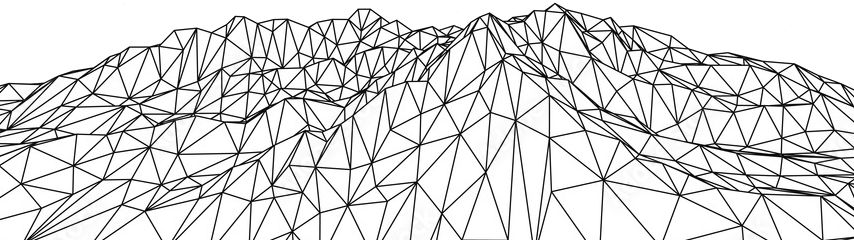
\includegraphics[width=\paperwidth]{../Unidad 2/Images/cover_bg}
\end{document}

\restoregeometry
\dominitoc[n]
\tableofcontents
\pagestyle{fancy}
\newpage
\mychapter{Unidad 1}
{\Large \alterfont \scshape En esta unidad estudiaremos \dots}
\minitoc\newpage

\thispagestyle{empty} \mbox{}

\newpage

\section{Este es el t\'itulo de la primera sección}
\boxabstract{Aprendizajes esperados:}{\blindtext}
\subsection{Imagina que la lección número uno tiene un t\'itulo muy, pero muy muy largo}

\begin{opening}\blindtext\end{opening}

\Blindtext

\begin{closing}\blindtext\end{closing}
\begin{problemas}\Blindenumerate[3]\end{problemas}
\newpage
\subsection{As\'i se llama la lección número dos}


\begin{opening}\blindtext\end{opening}

\Blindtext

\begin{closing}\blindtext\end{closing}




\newpage

\thispagestyle{plain}
\section{Secci\'on 2}
\boxabstract[fill=colorrds!10]{Aprendizajes:}{\blindtext}
\subsection{Nombre corto}


\begin{opening}\blindtext\end{opening}

\Blindtext

\begin{closing}\blindtext\end{closing}
\newpage
\subsection{Lecci\'on 2}

\begin{opening}\blindtext\end{opening}
\subsubsection{First subsubsection}
\Blindtext
\begin{important}[0.45\textwidth]{Conocimiento Clave}
    \blindtext
\end{important}
\Blindtext
\subsubsection{Second subsubsection}
\Blindtext
\subsubsection{Third subsubsection}
\Blindtext
\begin{closing}
    \blindtext
\end{closing}

\begin{problemas}
    \Blindenumerate[2]
\end{problemas}


\newpage
\mychapter{Unidad 2}
{\Large \alterfont \scshape En esta unidad estudiaremos \dots}
\minitoc\newpage

\thispagestyle{empty} \mbox{}

\newpage

\section{Este es el t\'itulo de la primera sección}
\boxabstract{Aprendizajes esperados:}{\blindtext}
\subsection{Imagina que la lección número uno tiene un t\'itulo muy, pero muy muy largo}

\begin{opening}\blindtext\end{opening}

\Blindtext

\begin{closing}\blindtext\end{closing}
\begin{problemas}\Blindenumerate[3]\end{problemas}
\newpage
\subsection{As\'i se llama la lección número dos}


\begin{opening}\blindtext\end{opening}

\Blindtext

\begin{closing}\blindtext\end{closing}




\newpage

\thispagestyle{plain}
\section{Secci\'on 2}
\boxabstract[fill=colorrds!10]{Aprendizajes:}{\blindtext}
\subsection{Nombre corto}


\begin{opening}\blindtext\end{opening}

\Blindtext

\begin{closing}\blindtext\end{closing}
\newpage
\subsection{Lecci\'on 2}

\begin{opening}\blindtext\end{opening}
\subsubsection{First subsubsection}
\Blindtext
\begin{important}[0.45\textwidth]{Conocimiento Clave}
    \blindtext
\end{important}
\Blindtext
\subsubsection{Second subsubsection}
\Blindtext
\subsubsection{Third subsubsection}
\Blindtext
\begin{closing}
    \blindtext
\end{closing}

\begin{problemas}
    \Blindenumerate[2]
\end{problemas}


\end{document}